\cleardoublepage

\chapter{Arquitecturas asimétricas y heterogéneas}
\label{ch:chapter2}

\section{Descripción general del paradigma big.LITTLE}

\subsection{Introducción a las arquitecturas asimétricas}
\label{sec:arch_asym}

Desde la aparición de los procesadores multinúcleo, y tras su auge durante la pasada
década como respuesta a las limitaciones en el incremento de la frecuencia de reloj
impuestas por la tecnología, este tipo de arquitecturas se han convertido en un pilar
clave en el desarrollo de arquitecturas de altas prestaciones, reuniendo a la vez
una gran capacidad de cálculo y una eficiencia energética notable.

Históricamente, los procesadores multinúcleo han estado formados por varias 
Unidades de Procesamiento (PUs), típicamente con idénticas características entre ellas.
Sin embargo, a medida que la ley de escalabilidad de Dennard~\cite{Den74} comienza a 
ver su fin, los sistemas heterogéneos se han convertido en las arquitecturas más 
atractivas en el campo de la computación de altas prestaciones. Este tipo de sistemas,
típicamente equipados con núcleos de procesamiento de propósito general y aceleradores
hardware de propósito específico, exhiben características, tanto desde el punto de vista
de las prestaciones como del consumo energético, que responden a las necesidades actuales
exigidas por los grandes problemas que surgen en diversos ámbitos de la ciencia y la
ingeniería.

Dentro de los sistemas heterogéneos es posible realizar una segunda clasificación en función de que los
distintos núcleos dispongan de distintos repertorios de instrucciones ({\em heterogeneous-ISA}) 
o utilicen el mismo repertorio de instrucciones ({\em single-ISA}). Estos últimos se denominan
habitualmente procesadores asimétricos ({\em asymmetric single-ISA CMP o ASISA-CMP})~\cite{survey_asym}.

En un procesador multinúcleo asimétrico (AMP), las diferencias entre los distintos núcleos se
deben a distinta microarquitecturas (asimetría física) o se trata de procesadores con la misma
microarquitectura pero distinta frecuencia o tamaño de cache (asimetría virtual). En ocasiones,
se usan técnicas de escalado dinámico de voltaje y frecuencia (DVFS) para emular procesadores 
asimétricos a partir de núcleos simétricos, consiguiendo así un sistema con asimetría virtual. Las
ventajas de este tipo de arquitecturas dependen del escenario en el que son utilizadas; en la 
actualidad, el uso de arquitecturas asimétricas es una tendencia en alza en el mercado de 
dipositivos móviles, en el que el tipo de tareas a ejecutar y su criticalidad es altamente 
heterogéneo, y el tiempo de vida de las baterías es un bien escaso y muy a tener en cuenta.

Dentro de las arquitecturas multinúcleo asimétricas, tienen especial relevancia los procesadores de la familia
ARM, que se denominan big.LITTLE para reflejar que incluyen procesadores potentes ({\em big})
junto con procesadores de menor rendimiento y mucho menor consumo ({\em LITTLE})[Jeff]. Por
ejemplo, se pueden combinar núcleos Cortex-A15 (big) con Cortex-A7 (LITTLE), si nos referimos al repertorio de
instrucciones de 32 bits (ARMv7), o Cortex A57 (big) con A53 (Little) para el caso de 64 bits
(ARMv8). Uno de los ejemplos reales más utilizados a día de hoy es el SoC Samsung Exynos (véase Figura~\ref{fig:exynos})
 en sus versiones de 32 y 64 bits, ampliamente utilizado en dispositivos móviles de última generación.

\begin{figure}[th!]
\begin{center}
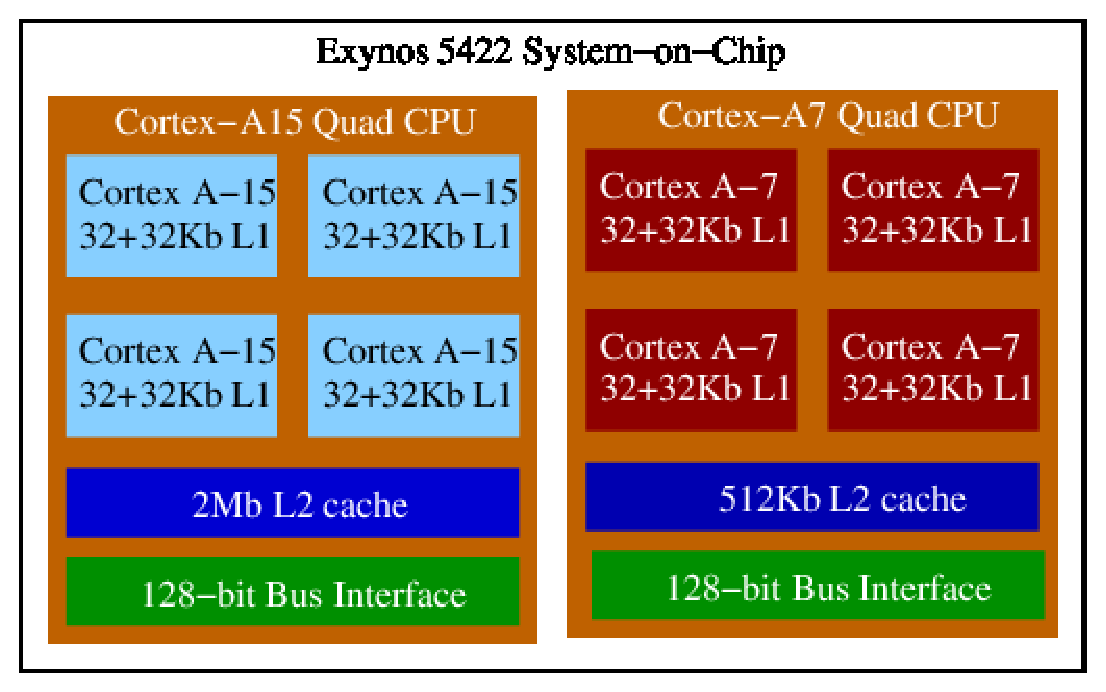
\includegraphics[width=0.4\columnwidth]{Figures/Exynos.eps}
\end{center}
\caption{\label{fig:exynos} Diagrama de bloques del SoC Samsung Exynos 5422.}
\end{figure}

En los últimos años, además, la utilización de este tipo de arquitecturas de muy bajo consumo se ha
convertido en un campo de investigación en pleno auge en la ruta hacia la construcción de futuros
supercomputadores que alcancen la barrera del Exaflop [REF ROAD TO EXAFLOP y MontBLANC]. La construcción
de este tipo de computadores y su posible idoneidad de cara a llegar a (y superar) dicha barrera
los ha convertido en un candidato más que factible a la hora de desarrollar técnicas y códigos
que exploten de manera eficiente todos los recursos computacionales que ofrecen.

\subsection{Soporte en el kernel para arquitecturas big.LITTLE}
\label{sec:models}

Las arquitecturas big.LITTLE modernas ofrecen un conjunto de distintos modelos de ejecución
soportados por el sistema operativo (algunos de ellos exigen soporte también a nivel de
hardware):

\begin{description}

	\item[Cluster Switching Mode (CSM)]

El procesador se divide de forma lógica en dos clusters, uno conteniendo los núcleos
rápidos, y otro conteniendo los núcleos lentos, pero sólo uno de ellos es utilizable
simultáneamente en tiempo de ejecución. El sistema operativo activa/desactiva los 
clusters de forma transparente, en función de la carga de trabajo, para equilibrar
el rendimiento y la eficiencia energética.

	\item[CPU migration (CPUM)]

Los núcleos físicos se agrupan en pares, cada uno formado por un núcleo rápido y otro
lento, construyendo {\em Núcleos Virtuales (VC)}, a los que el sistema operativo mapea
hebras. En un instante determinado, sólo un núcleo físico está activo por VC, dependiendo
de los requisitos exigidos por la carga computacional activa. En aquellas implementaciones
big.LITTLE en las que el número de núcleos lentos y rápidos no es el mismo, cada VC puede
estar formado por diferente número de núcleos de cada tipo. La solución implementada
por Linaro en el kernel de Linux se conoce como {\em In-Kernel Switcher (IKS)}~\cite{}.

	\item[Global Task Scheduling (GTS)]

Se trata del modelo más flexible. Todos los núcleos (lentos y rápidos) están disponibles
para la planificación de hebras, y el sistema operativo las mapea en función de la naturaleza
de la carga computacional asociada a cada uno de ellos y la disponibilidad de núcleos. 

\end{description}

\begin{figure}%[tbh!]
 \centering
  \begin{subfigure}{.75\textwidth}
   \centering
   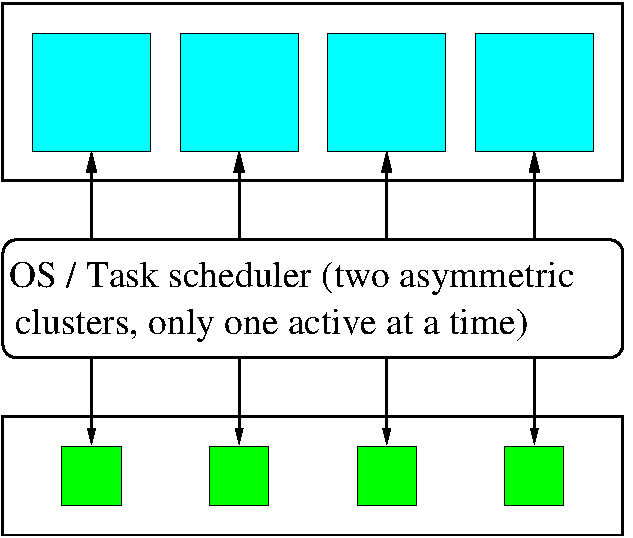
\includegraphics[width=0.4\textwidth]{Figures/Models/clustered.pdf}
   \caption{CSM}
  \end{subfigure}

	\medskip

  \begin{subfigure}{.75\textwidth}
   \centering
   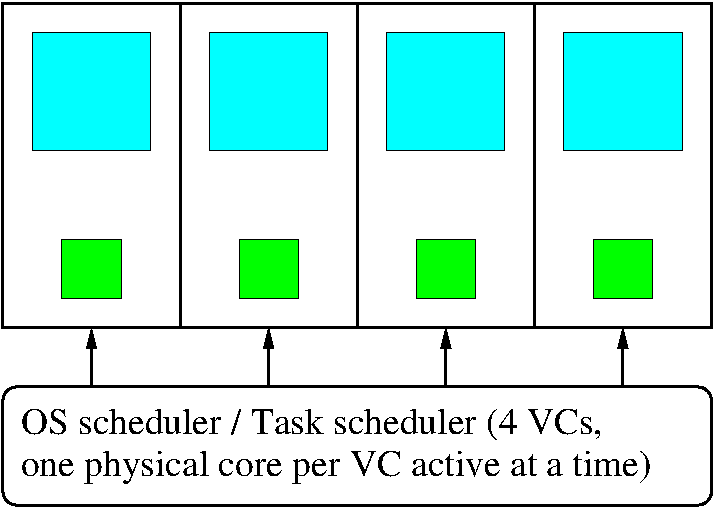
\includegraphics[width=0.45\textwidth]{Figures/Models/iks.pdf}
   \caption{CPUM}
  \end{subfigure}

	\medskip

  \begin{subfigure}{.75\textwidth}
   \centering
   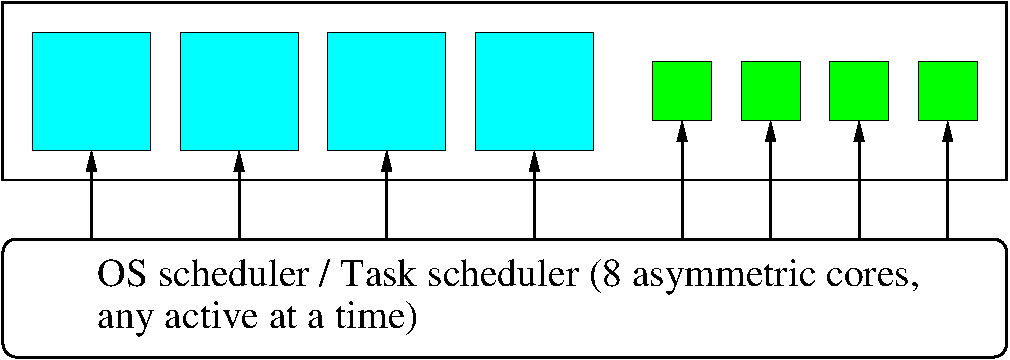
\includegraphics[width=0.6\textwidth]{Figures/Models/gts.pdf}
   \caption{GTS}
  \end{subfigure}
   \caption{Modos de operación de las arquitecturas big.LITTLE actuales.}
   \label{fig:modes}
\end{figure}

\comentario{Falta traducir figura}


La Figura~\ref{fig:modes} ofrece una visión esquemática de estos tres modelos de ejecución
sobre arquitecturas big.LITTLE modernas. GTS es la solución más flexible, ya que permite al planificador
del sistema operativo asignar hebras a cualquiera de los núcleos disponibles, es decir, todos
los núcleos disponibles se ofrecen al sistema operativo como candidatos a ejecutar el código
de cualquier hebra, independientemente de su naturaleza o características. Esta característica
permite migrar de forma muy sencilla aplicaciones multihebra ya existentes, incluyendo planificadores
de tareas en tiempo de ejecución, y explotar todos los recursos computacionales en este tipo de 
procesadores asimétricos, utilizando cualquier mecanismo estándar de creación y gestión de hebras
(por ejemplo, pthreads u OpenMP). Sin embargo, conseguir prestaciones óptimas no resulta tan
sencillo, especialmente en aplicaciones multihebra en las que el desequilibrio de carga introducido
por la asimetría de la arquitectura puede penalizar el rendimiento obtenido. Solucionar este problema
es uno de los objetivos de este trabajo.

De forma alternativa, CPUM propone una visión pseudosimétrica del procesador big.LITTLE; por ejemplo,
en el caso del SoC Exynos 5422, los 8 núcleos asimétricos son vistos de forma lógica como 4 grupos
de pares de procesadores, convirtiendo así la arquitectura en un sistema simétrico formado por
4 núcleos virtuales (VC), que son expuestos de esta manera al sistema operativo.

En la práctica, los planificadores de tareas en tiempo de ejecución pueden aproximar a nivel software
cualquiera de estos tres paradigmas. Un modelo trivial puede seguir las directivas de GTS para asignar
cualquier tarea lista para su ejecución a cualquiera de los núcleos disponibles en el sistema. Con esta
solución, el desequilibrio de carga podría resolverse desarrollando políticas de planificación a nivel
de tarea específicas (conscientes de la asimetría), para asignar tareas al recurso más apropiado en 
función de sus características. 

Sin embargo, este trabajo propone un enfoque alternativo, en el que el SoC asimétrico es visto de forma
lógica como un conjunto {\em simétrico} de núcleos virtuales, cada uno de ellos compuesto internamente
por distintos tipos de núcleo, pero considerado, de cara al planificador, como un sistema simétrico. Esto
facilita el desarrollo de políticas de planificación, como se verá más adelante, y permite incluso
reutilizar planificadores ya existentes sobre este tipo de arquitecturas.

\section{Descripción del entorno experimental}

Durante el presente trabajo se han utilizado dos plataformas distintas basadas en el paradigma big.LITTLE de ARM.
Se describen a continuación sus principales características, así como detalles adicionales acerca del software 
utilizado y el entorno experimental para la medición de consumo usado en parte del trabajo.

\subsection{Plataformas hardware evaluadas}

\subsubsection{\odroid}

\odroid es una

\subsubsection{\juno}

\subsection{Software utilizado}

\subsection{Entorno de medición de consumo}

Para el desarrollo del Capítulo~\ref{ch:chapter5} se han utilizado dos entornos experimentales de medición de consumo
energético sobre las plataformas \odroid y \juno. Ambos entornos se basan en sendas adaptaciones del software {\tt pmlib}~\cite{pmlib},
desarrollado por la Universidad Jaume I de Castellón; dicha herramienta, desarrollada en lenguaje Python, implementa un paradigma
 cliente/servidor, en el que la parte servidora se encarga de recoger continuamente muestras de potencia instantánea disipada
por cierto dispositivo, mientras que la utilización de una API propia permite instrumentar los códigos a perfilar desde el
punto de vista energético, que actúan como cliente realizando peticiones al servidor {\tt pmlib}.

Ambos entornos difieren en la forma en la que las muestras de consumo energético son recogidas desde el sistema objetivo:

\begin{description}

\item[\odroid:] El servidor {\tt pmlib} ha sido adaptado para interactuar con los sensores de consumo energético integrados 
en la placa y basados en resistencias de {\em shunt}. Dichos sensores ofrecen lecturas independientes para el consumo energético
del cluster formado por los Cortex-A7, Cortex-A15, GPU y RAM, con una frecuencia de refresco de cuatro muestras por segundo.

\item[\juno:] El servidor {\tt pmlib} ha sido adaptado para recoger los datos de consumo desde un DAQ XX fabricado por National
Instruments. Dicho dispositivo, a su vez, recoge muestras de potencia instantánea a partir de las resistencias de {\em shunt}
integradas en la plataforma, con lecturas actualizadas cada XX segundos e independientes para el cluster formado por los 
Cortex-A53, Cortex-A57, GPU y resto del sistema.

\end{description}

%-- Configuraciones para emacs --
%%% Local Variables:
%%% mode: latex
%%% TeX-master: "./principal.tex"
%%% End:
